% !TEX root =  ../../thesis.tex 

\chapter{Bayesian paradigm}
\label{ch : bayesian_paradigm}

\section{The bayesian motivation: A toy example}
To explain the motivation behind the bayesian paradigm, we will use an informal approach via the following toy example. Suppose there are three people A,B and C of whom A and B each are captains of a cricket team and C is the refree who tosses the coin. Given the importance of the toss in this sport each side would like to win the toss. Let us assume that based on experiences of an old friend captain B gets to know that the referee purposefully attempts at getting a heads on the toss. However given the nature of this problem, it is hard to quantify this belief in a single real number. Instead a belief that there is a 70 to 90\% chance that the result will be a heads is more likely than a belief that there is exactly an 80\% chance for the same. One might also have a slightly vague belief that there is more than 50\% chance that the toss will result into a heads. \\

\begin{figure}
	\centering
	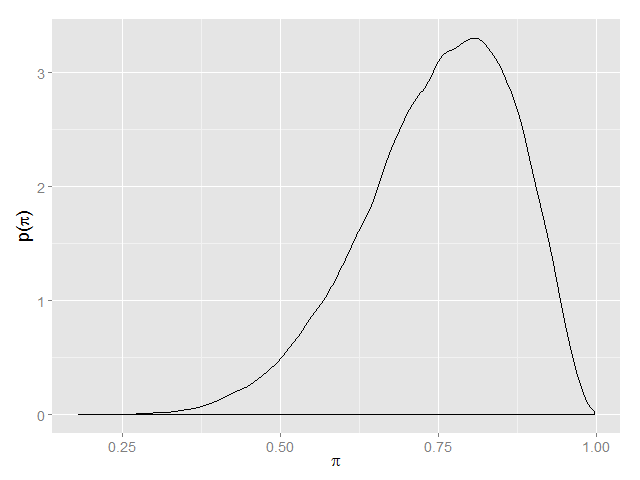
\includegraphics[scale=0.5]{mainmatter/chapter_2_bayesian_paradigm/toy_problem_pdf.png}
	\caption{PDF of the probability of getting heads on coin toss ($\pi$)}
	\label{fig : toy_problem_pdf}
\end{figure}


While subjective, these beliefs represent the prior probability distribution of a random variable in bayesian paradigm. In our toy 
problem the random variable is probability $\pi$ of getting a heads. For e.g. in \ref{fig : toy_problem_pdf} we can see one such prior distribution corresponding to the belief that the chance of getting a heads on toss is more than tails and it is more likely to be somewhere between 70 to 90\%. This is in contrast to the frequentist paradigm where the prior probability of getting a heads is a constant. However one can also model the frequentist scenario in bayesian paradigm by having all the probability mass at one single point (e.g. Direc delta distribution). 

\todo[inline]{talk about posterio and then introduce to the 2. bayes theorem, 3. bayesian software and MCMC methods }
